\section{Clientsoftware}
\label{sec:frontend}

\iffalse
- viele Anforderungen
- Fokus der Thesis
- beschreibt alle Schritte um eine Webandwendung in eine gelunge Kioskapplikation zu bringen
- Was meint Frontend: die eigentliche Kioskapplikation, Plattform: die Umgebung der Applikation, Deployment der Applikation
- SPA Routing im Frontend
- rein mit Webtechnologien, und noch weiter rein mit Browsertechnologien: beschränken auf HTML, CSS und JS
- mit Electron bindet man sich an die Plattform
\fi

Im Folgenden wird die Clientsoftware des Kiosksystems betrachtet. Damit ist der 
Softwareteil des Systems gemeint, welcher auf der Kiosk-Workstation vor 
Ort läuft. Diese wird in diesem Kapitel zur weiteren Betrachtung 
weiter unterteilt. Zum ersten in die \emph{Applikation}, 
also die eigentliche den Nutzer*innen zugängliche Kioskapplikation.
Zum zweiten in die \emph{Plattform} der Clientsoftware.
Also die Umgebung, in welcher die Applikation läuft.
Und schließlich wird das \emph{Deployment} besprochen -- also die Art wie die Applikation und 
Updates dieser auf die Kiosk-Workstation gelangen.\\

\subsection{Applikation}
\label{subs:applikation}

Anforderungen aus \autoref{chap:anforderungen}, welche die eigentliche Applikation 
der Clientsoftware betreffen, sind die Anforderungen \ref{nfa2}, \ref{nfa3} und \ref{nfa8}.\\

\ref{nfa8} stellt die Anforderung der Modularität an das gesamte Softwaresystem. Diese
betrifft also auch die Clientanwendung. Wie in \autoref{sec:backend} bereits erläutert, 
ist für eine starke Modularität eine lose Kopplung von Daten- und Präsentationsschicht ein
wichtiger Faktor. Umgekehrt bedeutet dies, dass die Clientanwendung eine in sich geschlossene
eigene Anwendung sein muss. Sie besitzt lediglich die Datenschnittstelle zum CMS. Das leistet im 
Falle der Webtechnologien eine Single-Page Applikation (SPA). Eine SPA wird einmalig von einem 
Server geladen. Laden von weiteren Seiten beim Navigieren durch die Oberfläche 
findet nicht statt \cite{js-definitive}. Um Transaktionen und neue Zustände möglich zu machen,
können jedoch im Hintergrund asynchrone Datenanfragen gestellt werden (AJAX). 
Die SPA gibt so den Nutzenden nicht mehr das Gefühl einer
Webseite, sondern einer geschlossenen Anwendung, was im Falle der Kiosksoftware ein gewünschter
Effekt ist und damit auch zur Erfüllung der Anforderung \ref{nfa4} beiträgt.\\
Das Laden einer einzigen Seite vom Server bedeutet jedoch nicht, dass keine Navigationsstruktur
mit Vor- und Zurück-Bewegungen implementieren werden kann. Die Navigation findet jedoch alleinig in 
der Clientanwendung statt und ist nicht mit Laden von neuen Seiten verbunden. Es werden lediglich
neue Zustände aufgerufen \cite{spa-manifesto}.\\

\ref{nfa2} fordert Offline-Verfügbarkeit. Auch hier trägt das Konzept der SPA zur 
Erbringung der Anforderung bei. Dadurch, dass die Anwendung nur einmal initial geladen werden muss 
und danach vollständig im Client zur Verfügung steht, ist eine Netzwerkverbindung nach dem initialen 
Laden nicht mehr nötig. Das umfasst allerdings nur die eigentliche Applikation und nicht die
AJAX-Anfragen, die auch zu späteren Zeitpunkten erfolgen können. Auch ist bei einem Neuladen
der Applikation immer eine Netzwerkverbindung zwingend nötig. Das Konzept der SPA erfüllt
die Anforderung der Offline-Verfügung also nur zu einem gewissen Teil. Allerdings bildet die Geschlossenheit
einer SPA eine wichtige Voraussetzung, um die Applikation auch vollständig offline zur Verfügung
zu stellen. \emph{Vollständig offline} meint hier also, dass auch Daten, die über
einen AJAX-Aufruf aus dem CMS geladen werden, lokal gecached werden können. Zwar wären Content-Daten bei
Offlinestatus nicht mehr durch das CMS aktualisierbar, aber zumindest die letzte Version solange verfügbar,
bis ein Netzwerkzugriff wieder möglich ist. Um solch einer Anforderung gerecht zu werden, bieten moderne 
Browser die Service-Worker API \cite{service-worker-api}.\\ 
Bei Service-Workern handelt es sich um Proxy-Server, welche sich zwischen der Webanwendung und dem 
Netzwerk befinden. Ein Service-Worker wird in einem Skript definiert, welches
unabhängig vom Prozess der Webseite ausgeführt wird \cite{service-worker-intro}. 
Dieses speichert Netzwerkzugriffe in einem lokalen Speicher und kann Anfragen auf
diesen verweisen, sollte das Netzwerk bei dem nächsten Zugriff nicht erreichbar sein \cite{service-worker-api}.
Service-Worker werden bei initialem Aufruf heruntergeladen und bleiben auch nach Schließen des Browsers
gespeichert. Das gilt auch für die Daten, welche sie speichern. Diese sind also auch bei Neustart ohne
Netzwerkverbindung noch vorhanden und können angezeigt werden.\\
Eine vollständige Offline-Verfügbarkeit wäre somit fast erreicht. Einzig Transaktionen, bei welchen Eingaben
und Daten von Nutzenden gespeichert werden sollen, können noch nicht offline verfügbar gemacht werden.
Auch hier kommt die Technik der Service-Worker an ihre Grenzen \cite{service-worker-post}.\\
Dennoch gibt es auch hier Lösungen für dieses
Problem. Beispielsweise bietet die JavaScript Datenbank pouchDB \cite{pouchdb} die Möglichkeit POST-Anfragen
und Dateien in einer lokalen Datenbank solange zu speichern, bis eine Netzwerkverbindung wiederhergestellt ist,
um sie dann mit einer Backend-Datenbank zu synchronisieren. Dieser Ansatz wird jedoch im Rahmen dieser Arbeit,
aus Gründen des Umfangs, nicht weiter verfolgt.\\

\ref{nfa8} fordert schließlich die Multilingualität der Oberfläche. Wie in \autoref{sec:backend} 
bereits erläutert, können Datensätze im CMS der \shst{} mehrsprachig angelegt werden. Diese Funktion
existiert bei den meisten CMS. Die Daten werden dann entweder über einen gemeinsamen Datensatz oder über einen
Datensatz für jede Sprache der Clientanwendung zur Verfügung gestellt. Die Oberfläche der Clientanwendung muss die Möglichkeit
bieten die Sprache umzustellen. Erfolgt dies, muss keine neue Seite vom Server sondern maximal ein anderer
Datensatz angefordert und die angezeigten Daten durch die entsprechende Sprachversion ausgetauscht werden.\\

\begin{figure}
    \centering
    \includestandalone[width=1\textwidth]{figures/plant/out/ss-app-class-diagram}
    \caption{Komponenten Diagram der \shst{} Clientanwendung}
    \label{fig:ss-app-class-diagram}
\end{figure}

Um dieser beschriebenen Architektur gerecht zu werden, wurden für die Clientanwendung der \shst{} 
unter Anderen die JavaScript Bibliotheken React \cite{react} und Redux \cite{redux} zusammen mit dem 
Toolkit Workbox \cite{workbox} verwendet. React bildet dabei
den Rahmen für die SPA-Architektur, Workbox bietet eine Bibliothek, die es erleichtert 
Service-Worker zu implementieren und Redux ist eine Bibliothek, die ein Pattern für die Verwaltung 
von Applikationszuständen bereitstellt. Bei steigender Komplexität von Zuständen in einer Anwendung 
bietet der Einsatz der Redux Bibliothek allerhand Vorteile 
-- dies ist im Rahmen dieser Thesis aber von untergeordneter Bedeutung und wird daher
nicht weiter erläutert.\\

React bietet die Möglichkeit, die meisten der zuvor genannten Anforderungen zu erfüllen. 
Das ist neben der Implementierung der SPA-Architektur, auch die Möglichkeit die 
Anwendung zu modularisieren. Denn: Neben der losen Kopplung von CMS und Clientanwendung
ist auch eine Modularität innerhalb der Clientanwendung nötig, um die Anforderung \ref{nfa8}
vollständig zu erfüllen. React erlaubt dies durch sein Komponenten-basiertes System. Einzelne
Interface-Elemente oder auch einzelne Unterseiten können als Komponenten gekapselt werden.
Wie fein diese Kapselung sein soll, kann von der entwickelnden Person entschieden werden. Richtig implementiert,
können Komponenten so wiederverwendet, ausgetauscht oder das System leicht um neue erweitert werden.\\
\autoref{fig:ss-app-class-diagram} zeigt die Komponentenstruktur der Clientanwendung der \shst{}.
Die Abbildung ist vereinfacht und zeigt nur die wichtigsten Komponenten. Die Art der Darstellung
orientiert sich dabei an der von \citeext{visualizing-react} vorgeschlagenen Weise um React Anwendungen
zu visualisieren. Diese wiederum basiert auf dem System des UML-Klassendiagramms \cite{uml-spec}, 
jedoch sind die Klassen in diesem Falle keine Klassen im Sinne der Objektorientierung, sondern die Komponenten 
\footnote{React-Komponenten können Klassen sein - müssen aber nicht. Seit React 16.8.0 und
der Einführung der Hook-API \cite{react-hooks} kann sogar gänzlich auf Klassen verzichtet werden und Komponenten 
durchgängig als Funktionen implementiert werden. Das wurde in diesem Falle so umgesetzt.}.
Rot markierte Komponenten sind Container-Komponenten und haben keine eigene Darstellung -- sie implementieren
lediglich Geschäftslogik. Blau markierte Komponenten sind Interface-Komponenten, die eine direkte 
Darstellung in der Oberfläche haben. Die einzelne gelb markierte Komponente ist der Redux-Store. 
Er ist ebenfalls eine besondere Art der Container-Komponente und beinhaltet den Applikationszustand. 
Die gestrichelten Linien visualisieren welche Komponenten dabei direkten Zugriff auf den 
Store haben.\\
Im Zentrum der Abbildung befindet sich die Router-Komponente. Diese entscheidet anhand der aufgerufenen
URL, welche Komponenten geladen und dargestellt werden. Teilbäume, abgehend von der Router-Komponente, können als
die Hauptmodule der Applikation gesehen werden. Sie können dabei Untermenüs oder Module sein, welche
die konkreten Funktionalitäten wie die Spenden-Funktion (\ref{fa3}) oder die Newsletter-Funktion (\ref{fa5}) 
implementieren. Diese klarer Abgrenzung der einzelnen Module bietet so die Möglichkeit, diese leicht
zu entfernen, durch andere zu ersetzen oder um neue zu erweitern.\\

\begin{figure}
  \lstinputlisting[%
    firstline=8,
    style=ES6, 
    caption=
  ]{data/sharing-station-app/webpack.prod.config.js}
  \caption{Ausschnitt der Webpack Konfiguration der \shst{} Clientanwendung}
  \label{fig:webpack-config}
\end{figure}

Workbox hilft bei der Implementierung von Service-Worker Skripten. Darüber hinaus gibt es ein 
Workbox-Plugin \cite{workbox-webpack-plugin} für den JavaScript-Bundler Webpack \cite{webpack}. 
Beide Technologien wurden im Falle der \shst{} eingesetzt. Mit Hilfe dieses Plugins müssen 
Service-Worker Skripte nicht selbst implementiert werden, sondern werden automatisiert erstellt.
In der Konfiguration von Webpack kann durch Setzen von Parametern bestimmt werden, was
der Service-Worker leisten soll. \autoref{fig:webpack-config} zeigt einen Teil der 
Webpack-Konfiguration der \shst{}. In Zeile 24-32 wird das Objekt zur Generierung des
Service-Workers erstellt. Als Parameter wird ein Objekt mit der Konfiguration übergeben. 
Dieses Objekt ist optional -- auch ohne Konfiguration würde ein Service-Worker erstellt werden,
welcher dafür sorgt, dass alle von Webpack erstellten Files beim Nutzen der Applikation
gecached und offline verfügbar gemacht werden. Weitere Funktionalitäten können durch
Setzen diverser Konfigurationsparameter aktiviert werden.\\
In Zeile 27 wird die maximale Dateigröße gesetzt. 
Dateien größer als dieser Wert, werden nicht offline verfügbar gemacht. Dieser Wert
ist standardmäßig niedriger und wurde an dieser Stelle erhöht, um auch das Video zu cachen, welches
für den Idle-Modus (\ref{fa8}) benötigt wird.

\begin{figure}
    \centering
    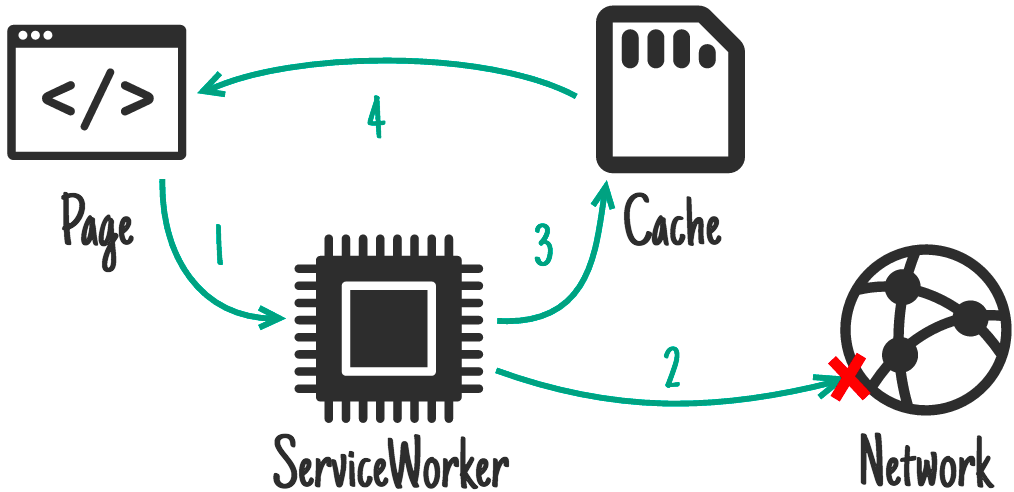
\includegraphics[width=1\textwidth]{figures/images/ss-network-falling-back-to-cache.png}
    \caption{Network first Strategie. Quelle: \cite{offline-cookbook}}
    \label{fig:network-first}
\end{figure}

In den Zeilen 28-31 wird definiert, welche Dateien, neben den von Webpack erstellten Dateien, 
gecached werden sollen. Das sind in diesem Fall alle Daten und Dateien, die durch Netzwerkanfragen an 
das CMS geladen werden. Diese Anfragen haben den gemeinsamen Namespace \texttt{/api/} und 
können dadurch mit dem regulären Ausdruck \texttt{/.*\textbackslash/api\textbackslash/.*/} erfasst werden.
Mit der Option \texttt{handler} wird eine Caching-Strategie gewählt. Workbox bietet hier die Möglichkeit
zwischen fünf verschiedenen, vordefinierten Handler-Klassen zu wählen \cite{workbox-strategies}. 
Die Strategie der Klasse \texttt{NetworkFirst} beruht darauf, dass die Anfrage zuerst an das Netzwerk
gestellt wird. Ist dieses nicht erreichbar, wird auf die letzte Version im Cache zurückgegriffen. 
Ist ein Netzwerkzugriff erfolgreich, wird auch immer die Version im Cache durch die neue Version ersetzt.
\autoref{fig:network-first} visualisiert diese Strategie.

\section{Plattform}
\label{sec:plattform}
\subsection{Deployment}
\label{subs:deployment}

Die einzige Anforderung, welches das Deployment direkt betrifft, ist die Anforderung
\ref{nfa7}. Diese besagt lediglich, dass dies möglichst einfach und von außerhalb möglich
sein soll.\\
Bei nativen Applikation wäre hier ein Updater denkbar. Also ein Service,
welcher regelmäßig die Verfügbarkeit neuer Versionen auf einem Server prüft und einen Download 
dieser anbietet. Electron.js bietet für diesen Fall einige Möglichkeiten, diesen Prozess 
möglichst simpel zu gestalten. Beispielsweise mit dem eigenen 
\texttt{autoUpdater}-Modul \cite{electron-autoUpdater} oder Plugins wie 
\emph{electron-builder} \cite{electron-builder}. Auch sind mit beiden Möglichkeiten
automatische Updates umsetzbar.\\
Im Falle einer Applikation, die einzig mit Browsertechnologien implementiert wurde, sind 
noch simplere Strategien denkbar. Hier ist ein normales Webhosting der Applikationsfiles 
bereits eine ausreichende Deployment-Strategie. Wurde keine Offline-Verfügbarkeit durch
Service-Worker implementiert, können die statischen Files einer Browseranwendung
auch einfach auf dem Filesystem der Workstation hinterlegt und in einem Browser aufgerufen 
werden. Eventuelle Updates müssten in diesem Falle aber vor Ort oder durch einen
Fernzugriff auf den Rechner eingespielt werden. Im Fall des Webhostings genügt das Überspielen
der neuen Files auf einen Webserver.\\

Für die \shst{} wurde auf dem Server neben dem CMS auch ein Webserver installiert, welcher die 
Applikationsfiles ausliefert (\autoref{fig:ss-deployment-diagram}). Zusätzlich wurde über den 
firmeninternen GitLab-Server \cite{gitlab} eine Build- und Deployment-Pipeline eingerichtet, welche die 
Applikationsfiles automatisch generiert und vom Master-Branch des Repositorys auf den Webserver überträgt. 
Für ein Updaten der Clientapplikation, auf der Workstation in der Ausstellung, ist also nichts weiter 
nötig als die Änderungen auf den Master-Branch des Repositorys zu übertragen und die Applikation vor
Ort neu zu laden.\\
Das Webhosting der Applikation bietet außerdem den Vorteil, dass diese jeder Zeit in einem Browser 
über das Internet aufgerufen werden kann. Beim Anlegen von Daten im CMS kann dies so als
Preview genutzt werden.
